% Page: Random experiments and probability
% sources/stat2003/chapters/prob-01-experiments.qmd
% Factories on that page. A is "defective" and B_i is "made in factory i".
% Width is the prior, height is the defect rate, and the area is the joint
% probability. Bayes' rule divides one area by the sum 0.029.
\documentclass[border=6pt]{standalone}
\usepackage[T1]{fontenc}
\usepackage{lmodern}
\usepackage{amsmath,amssymb}
\usepackage{tikz}
\usetikzlibrary{calc}
\usepackage{pgfplots}
\pgfplotsset{compat=1.18}
\definecolor{ink}{HTML}{1F2430}
\definecolor{statblue}{HTML}{174A7E}
\definecolor{bluefill}{HTML}{D7E5F0}
\definecolor{accent}{HTML}{9C4A32}
\definecolor{accentfill}{HTML}{F4E4DC}
\definecolor{grey}{HTML}{5E6A75}
\definecolor{greyfill}{HTML}{E6EAEE}
\pgfplotsset{
  stat/.style={
    scale only axis,
    axis lines=left,
    axis line style={ink, line width=0.6pt},
    tick style={ink, line width=0.45pt},
    tick label style={font=\small, text=ink},
    label style={font=\small, text=ink},
    title style={font=\small, text=ink, align=center},
    clip=false,
    unbounded coords=jump,
    scaled ticks=false,
  },
}
\begin{document}
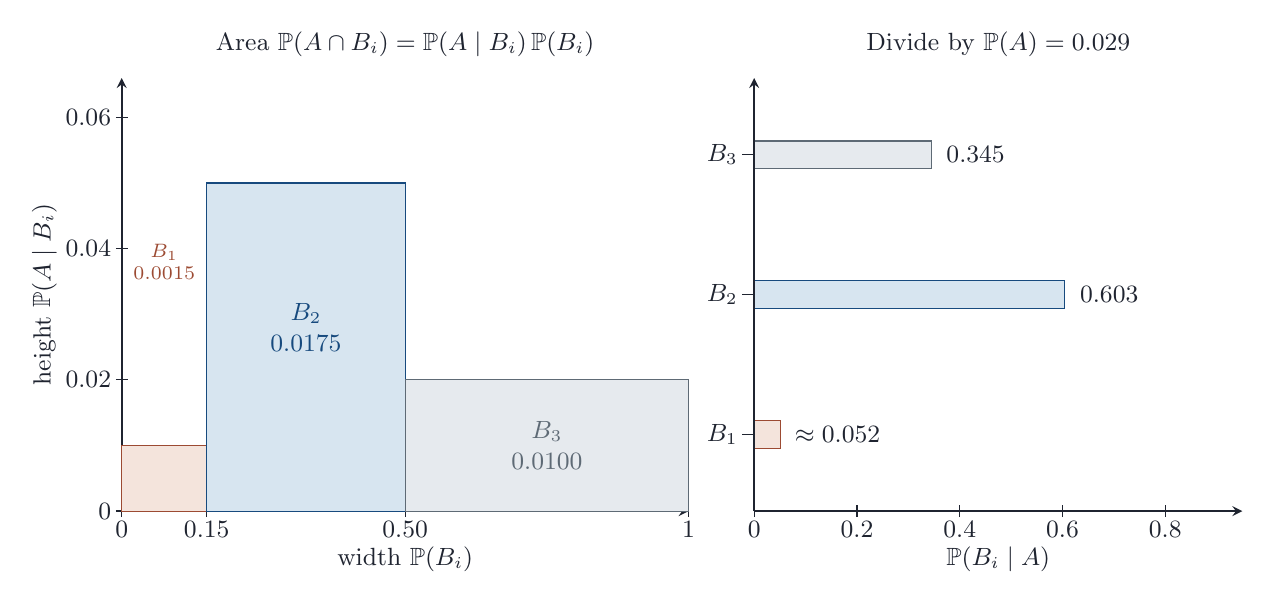
\begin{tikzpicture}[every node/.style={text=ink, inner sep=1.5pt}]
\begin{axis}[
  stat, width=7.2cm, height=5.5cm, name=areas,
  xmin=0, xmax=1, ymin=0, ymax=0.066,
  xtick={0,0.15,0.50,1},
  xticklabels={$0$,$0.15$,$0.50$,$1$},
  ytick={0,0.02,0.04,0.06},
  yticklabels={$0$,$0.02$,$0.04$,$0.06$},
  xlabel={width $\mathbb{P}(B_i)$},
  ylabel={height $\mathbb{P}(A\mid B_i)$},
  title={Area $\mathbb{P}(A\cap B_i)=\mathbb{P}(A\mid B_i)\,\mathbb{P}(B_i)$},
]
  \fill[accentfill] (axis cs:0,0) rectangle (axis cs:0.15,0.01);
  \fill[bluefill] (axis cs:0.15,0) rectangle (axis cs:0.50,0.05);
  \fill[greyfill] (axis cs:0.50,0) rectangle (axis cs:1,0.02);
  \draw[accent, thin] (axis cs:0,0) rectangle (axis cs:0.15,0.01);
  \draw[statblue, thin] (axis cs:0.15,0) rectangle (axis cs:0.50,0.05);
  \draw[grey, thin] (axis cs:0.50,0) rectangle (axis cs:1,0.02);
  \node[font=\scriptsize, align=center, accent] at (axis cs:0.075,0.038)
    {$B_1$\\$0.0015$};
  \node[font=\small, align=center, statblue] at (axis cs:0.325,0.028)
    {$B_2$\\$0.0175$};
  \node[font=\small, align=center, grey] at (axis cs:0.75,0.010)
    {$B_3$\\$0.0100$};
\end{axis}

\begin{axis}[
  stat, width=6.2cm, height=5.5cm,
  at={($(areas.outer north east)+(1.25,0)$)}, anchor=outer north west,
  xmin=0, xmax=0.95, ymin=0.45, ymax=3.55,
  xtick={0,0.2,0.4,0.6,0.8},
  ytick={1,2,3},
  yticklabels={$B_1$,$B_2$,$B_3$},
  xlabel={$\mathbb{P}(B_i\mid A)$},
  title={Divide by $\mathbb{P}(A)=0.029$},
  xbar, bar shift=0pt, bar width=10pt,
  axis on top,
]
  \addplot[fill=accentfill, draw=accent, thin] coordinates {(0.051724,1)};
  \addplot[fill=bluefill, draw=statblue, thin] coordinates {(0.603448,2)};
  \addplot[fill=greyfill, draw=grey, thin] coordinates {(0.344828,3)};
  \node[font=\small, anchor=west] at (axis cs:0.07,1) {$\approx 0.052$};
  \node[font=\small, anchor=west] at (axis cs:0.625,2) {$0.603$};
  \node[font=\small, anchor=west] at (axis cs:0.365,3) {$0.345$};
\end{axis}
\end{tikzpicture}
\end{document}
